\section{Devices connection}

Due to the last two \direct features described in the previous section, devices cannot create and destroy connection opportunistically, so for our simulation we had to 
%introduce a connection establishing phase which creates a \direct group and provides to all the devices a complete address map to let them communicate.
manually create a \direct \textit{group} and also to provide devices a complete address map, in order to let them communicate with each
devices.
Connection setup consists of the following operations:
	\begin{itemize}
		\item One of the devices asks other devices for connection
		\item When a device accepts, it starts a DHCP negotiation with the device which started the connection. If no \direct group exists, a group is created and the device which started the connection becomes the \textit{group owner}. If requesting device is already an owner of a pre-existing group, target device is added to this group. At the end of this phase, each device has an IP address, but only group owner's IP is available via \direct APIs. 
		\item Each device opens a \textit{TCP Server Socket} on port 8888, listening for incoming connections.
		\item When a device connects to a group, it sends a \textit{Ping message} to the \textit{group owner} via a socket. This kind of message is used by the \textit{group owner} to collect MAC and IP addresses of all devices in the group: MAC address is included into the \emph{Ping message} by each device, the second is obtained by the receiver from the incoming Socket information (using Java APIs).
		\item After collecting all the pairs composed by \begin{center}\tt{<MAC address,IP address>}\end{center} from all the devices in the group, \textit{group owner} creates a map, and sends it broadcast, to let devices communicate directly.
	\end{itemize}
	
Once that all these operations have been done, all the devices are connected and can communicate each other directly via TCP Sockets. An example of a created network is visible in figure \ref{fig:device_network}.

\begin{figure}[!htbp]
\centering
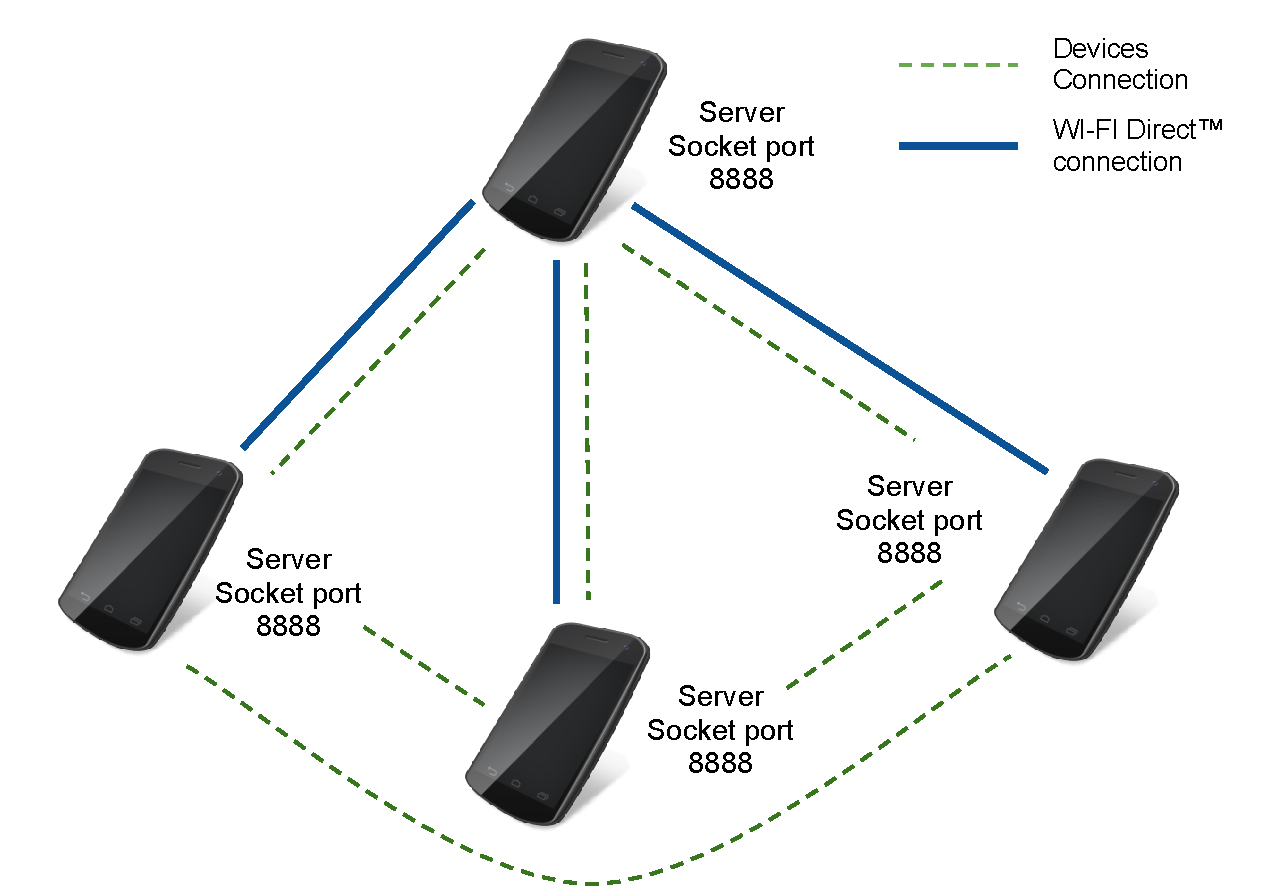
\includegraphics[width=3.6in]{imgs/Devices_network.pdf}
\caption{Network of four devices. Blu lines indicates the \direct group topology, and green lines the logical network}
\label{fig:device_network}
\end{figure}
